\documentclass{article}
\usepackage{amsmath}
\usepackage{amssymb}
\usepackage[a4paper, top=25mm, bottom=25mm, left=25mm, right=25mm]{geometry}
\usepackage{pgfplots}
\pgfplotsset{compat=1.18}
\usepackage{mathtools}
\usepgfplotslibrary{polar}
\usepgfplotslibrary{fillbetween}

\begin{document}
\pagestyle{empty}
\large

\begin{center}
2023-2024 Fall \\MAT124 Resit\\(29/01/2024)
\end{center}

\noindent 1.

\hfill

\noindent (a) Find the critical points of the function
\[f(x,y)=4x^3-6xy+y^2+2y\]
\noindent and classify them.

\hfill

\noindent (b) Find the maximum and minimum values of the function
\[f(x,y,z)=x+y+z\]

\noindent by using Lagrange multipliers on the ellipsoid $x^2+4y^2+9z^2=1764$.

\hfill

\noindent 2.

\hfill

\noindent (a) Sketch the domain of integration and rewrite the integral by changing the order of integration.

\[\int_0^1\int_0^{x\sqrt3}\mathrm{e}^{-x^2-y^2}\,dy\,dx+\int_1^2\int_0^{\sqrt{4-x^2}}\mathrm{e}^{-x^2-y^2}\,dy\,dx\]

\hfill

\noindent (b) Evaluate the integral
\[\iint_R\frac{xy}{1+x^4}\,dA\]

\noindent where $R$ is the triangle with vertices $(0,0),\:(1,0)$ and $(1,1)$.

\hfill

\noindent 3. The following integral gives the volume of the region that lies inside the sphere $x^2+y^2+z^2=4$ and between the planes $z=0$ and $z=1$.
\[V=4\int_0^{\pi/2}\int_0^{\sqrt3}\int_0^1r\,dz\,dr\,d\theta+4\int_0^{\pi/2}\int_{\sqrt3}^2\int_0^{\sqrt{4-r^2}}r\,dz\,dr\,d\theta\]

\hfill

\noindent (a) Write the integral in rectangular coordinates with the order of integration $dz\,dy\,dx$.

\hfill

\noindent (b) Write the integral in spherical coordinates.

\hfill

\noindent 4.

\hfill

\noindent (a) Is $\mathbf{F}(x,y)=2xy\sin\left(x^2y\right)\mathbf{i}-x^2\sin\left(x^2y\right)\mathbf{j}$ conservative? Why?

\hfill

\noindent (b) Show that

\[\mathbf{F}(x,y,z)=\left(2x+y^2+z\cos x\right)\mathbf{i}+\left(2xy+\mathrm{e}^z\right)\mathbf{j}+\left(1+y\mathrm{e}^z+\sin x\right)\mathbf{k}\]

\hfill

\noindent is conservative.

\hfill

\noindent (c) Find its potential function.

\newpage

\noindent 5. $\mathbf{F}(x,y,z)=\left(2x+y^2+z\cos x\right)\mathbf{i}+\left(2xy+\mathrm{e}^z\right)\mathbf{j}+\left(1+y\mathrm{e}^z+\sin x\right)\mathbf{k}$

\hfill

\noindent (a) Let $C $ be the curve of intersection of the cone $z^2=4x^2+9y^2$ and the plane $z=1+x+2y$, and let $D$ be the part of the curve $C$ that lies in the first octant $x\geq0,\:y\geq0,\:z\geq0$ from $(1,0,2)$ to $(0,1,3)$. Evaluate $\int_D\mathbf{F}\cdot d\mathbf{r}$.

\hfill

\noindent (b) Let $C$ be the curve of intersection of $x^2+y^2=1$ and $z=40$. Evaluate $\int_C\mathbf{F}\cdot d\mathbf{r}$.

\hfill

\noindent 6. Evaluate

\[\oint_C\left(x^3\sin\left(\sqrt{x^2+4}\right)-x\mathrm{e}^{x+2y}\right)\,dx + \left(\cos\left(y^3+y\right)-4y\mathrm{e}^{x+2y}\right)\,dy\]

\hfill

\noindent where $C$ is the counterclockwise boundary of the parallelogram with vertices $(2,0)$, $(0,-1)$, $(-2,0)$, and $(0,1)$.

\newpage

\begin{center}
2023-2024 Fall Resit (29/01/2024) Solutions\\
(Last update: 8/7/25 (7th of August) 3:33 PM)
\end{center}

\noindent 1.

\hfill

\noindent (a) To find the critical points of $f$, determine where both $f_x=f_y=0$ or one of the partial derivatives does not exist.

\[f_x=12x^2-6y,\quad f_y=-6x+2y+2\]

\[f_x=0\implies y=2x^2,\quad f_y=0\implies y=3x-1\]
\[f_x=f_y=0\implies 2x^2-3x+1=0\implies x_{1,2}=\frac{3\pm\sqrt{(-3)^2-4\cdot2\cdot 1}}{2\cdot2}=\frac{3\pm1}{4}\]

\[x=\frac12\implies y=2\cdot\left(\frac12\right)^2=\frac12,\quad x=1\implies y=2\cdot(1)^2=2\]

\hfill

\noindent The critical points occur at $\left(1/2,1/2\right)$ and $(1,2)$. To classify these points, apply the second derivative test.

\[f_{xx}=24x,\quad f_{xy}=f_{yx}=-6,\quad f_{yy}=2\]

\hfill

\noindent Calculate the Hessian determinant at these points.

\[\left|\begin{array}{cc}
f_{xx}&f_{xy}\\
f_{yx}&f_{yy}
\end{array}\right|=f_{xx}f_{yy}-f_{xy}^2\]

\hfill

\[(1/2,1/2)\quad\rightarrow\quad\begin{array}{l}f_{xx}=12,\quad f_{xy}=f_{yx}=-6,\quad f_{yy}=2\\[1em]
f_{xx}f_{yy}-f_{xy}^2=12\cdot2-(-6)^2=-12<0\quad\end{array}\]

\hfill

\[(1,2)\quad\rightarrow\quad\begin{array}{l}f_{xx}=24,\quad f_{xy}=f_{yx}=-6,\quad f_{yy}=2\\[1em]f_{xx}f_{yy}-f_{xy}^2=24\cdot2-(-6)^2=12>0,\quad f_{xx}>0\end{array}\]

\hfill

\[\boxed{\text{A local min occurs at } (1,2) \text{ and a saddle point occurs at } (1/2,1/2).}\]

\hfill

\noindent (b) Let $g(x,y,z)=x^2+4y^2+9z^2-1764$ be the constraint. Then solve the system of equations below.

\[
\left.
\begin{array}{ll}
\displaystyle\nabla f=\lambda\nabla g\\
\displaystyle g(x,y,z)=0
\end{array}
\right\}\quad
\begin{array}{ll}
\nabla f=\left\langle1,1,1\right\rangle=\lambda\left\langle2x,8y,18z\right\rangle=\lambda\nabla g\\[1em]\displaystyle\therefore x=\frac1{2\lambda},\quad y=\frac1{8\lambda},\quad z=\frac1{18\lambda}
\end{array}
\]

\hfill

\noindent Use the constraint.

\begin{align*}x^2+4y^2+9z^2-1764=0&\implies\left(\frac1{2\lambda}\right)^2+4\left(\frac1{8\lambda}\right)^2+9\left(\frac1{18\lambda}\right)^2=1764\\\\&\implies \frac{49}{144\lambda^2}=42^2\implies\lambda=\pm\frac1{72}\end{align*}

\[\lambda=\pm\frac1{72}\implies x=\pm36,\quad y=\pm9,\quad z=\pm4\]

\hfill

\noindent To find the minimum and maximum values, consider the points $(-36,-9,-4)$ and $(36,9,4)$, respectively.

\[\boxed{f_{\text{min}}=-36-9-4=-49,\quad f_{\text{max}}=36+9+4=49}\]

\hfill

\noindent Compare all the values.

\[f(0,y,z)=f(x,0,z)=f(x,y,0)=0,\quad f\left(\frac14,\frac14,\frac12\right)=\frac14\cdot\frac14\cdot\left(\frac12\right)^2=\frac1{64}\]

\[\boxed{\text{The maximum value is }\frac1{64},\text{ the minimum value is }0.}\]

\hfill

\noindent 2.

\hfill

\noindent (a)
\begin{center}
\begin{minipage}{0.5\textwidth}
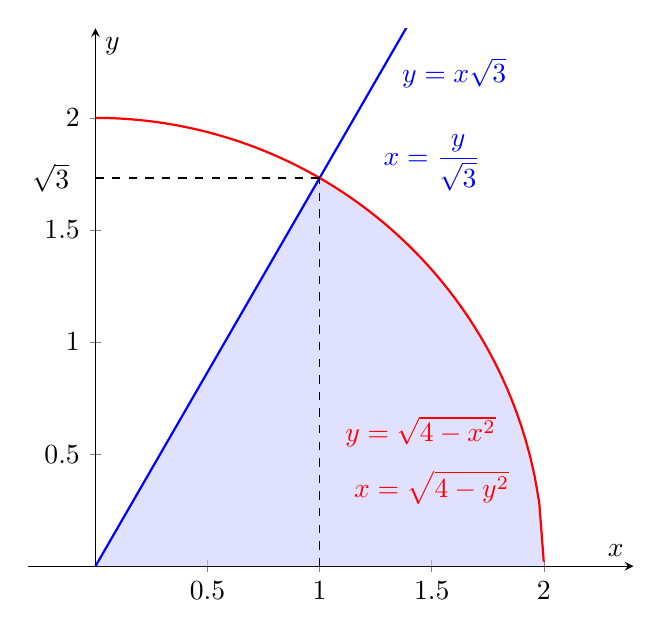
\begin{tikzpicture}
  \begin{axis}[
    axis equal image,
    xlabel=$x$, ylabel=$y$,
    xmin=-0.3, xmax=2.4,
    ymin=0, ymax=2.4,
    domain=0:1.2,
    samples=100,
    axis lines=middle,
    clip=true,
    scale=1.2,
    ]

    \addplot [name path=A, domain=0:2, draw=none] {min(x*sqrt(3),sqrt(4-x^2))};
    \addplot [name path=B, domain=0:2, draw=none] {0};
    \addplot [fill=blue!20, opacity=0.6] fill between[of=A and B];

    \addplot [blue, thick, domain=0:2] {x*sqrt(3)};
    \addplot [red, thick, domain=0:2] {sqrt(4-x^2)};
    
    \draw[dashed] (1,0)--(1,1.732); \draw[dashed] (0,1.732)--(1,1.732);
    
    \node[red] at (1.45,0.6) {$y=\sqrt{4-x^2}$};
    \node[red] at (1.5,0.35) {$x=\sqrt{4-y^2}$};
    \node[blue] at (1.6,2.2) {$y=x\sqrt3$};
    \node[blue] at (1.5,1.8) {$\displaystyle x=\frac y{\sqrt3}$};
    \node at (-0.2,1.732) {$\sqrt3$};
  \end{axis}
\end{tikzpicture}
\end{minipage}
\begin{minipage}{0.45\textwidth}
\[\boxed{\int_0^{\sqrt3}\int_{y/\sqrt3}^{\sqrt{4-y^2}}\mathrm{e}^{-x^2-y^2}\,dx\,dy}\]
\end{minipage}
\end{center}

\hfill

\noindent (b) Sketch the region.

\hfill

\begin{center}
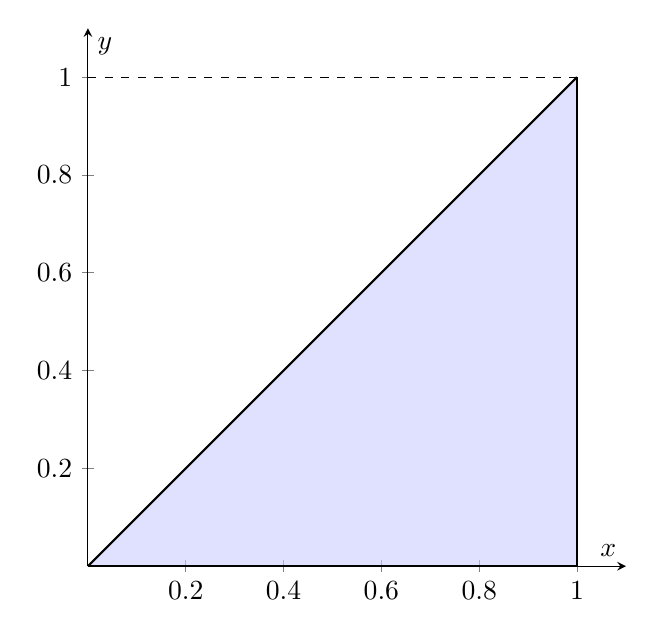
\begin{tikzpicture}
  \begin{axis}[
    axis equal image,
    xlabel=$x$, ylabel=$y$,
    xmin=0, xmax=1.1,
    ymin=0, ymax=1.1,
    domain=0:1.5,
    samples=100,
    axis lines=center,
    clip=true,
    scale=1.2,
    ]
    
    \addplot [domain=0:1, thick] {x};
    \addplot [domain=0:1, thick] {0};
    \draw (1,0)--(1,1);
    
    \addplot [domain=0:1, draw=none, name path=A] {x};
    \addplot [domain=0:1, draw=none, name path=B] {0};

    \addplot [fill=blue!20, opacity=0.6] fill between[of=A and B];

    \draw[dashed] (0,1)--(1,1);
  \end{axis}
\end{tikzpicture}
\end{center}

\hfill

\begin{align*}\iint_R\frac{xy}{1+x^4}\,dA&=\int_0^1\int_0^x\frac{xy}{1+x^4}\,dy\,dx=\int_0^1\frac x{1+x^4}\bigg[\frac{y^2}2\bigg]_{y=0}^{y=x}\,dx=\frac12\int_0^1\frac{x^3}{1+x^4}\,dx\\\\&=\frac12\cdot\bigg[\frac14\ln\left|1+x^4\right|\bigg]_0^1=\frac12\cdot\frac14\left(\ln2-\ln1\right)=\boxed{\frac18\ln2}\end{align*}

\hfill

\noindent 3.

\hfill

\noindent (a)
\[
\begin{array}{c}
z=z\\
x=r\cos\theta\\
y=r\sin\theta\\
r^2=x^2+y^2\\
dV=r\,dz\,dr\,d\theta=dz\,dy\,dx
\end{array}\quad\rightarrow\quad
\begin{array}{c}
z=\sqrt{4-r^2}\implies z=\sqrt{4-x^2-y^2}\\
z=1
\end{array}
\]

\hfill

\noindent Notice that we have two distinct upper bounds for $z$, which are $z=\sqrt{4-x^2-y^2}$ and $z=1$. The lower bound for $z$ is $z=0$. For the upper bounds of $z$, we choose the minimum of the bounds. If we project the shape onto the $xy$-plane, we get $x^2+y^2=4$. Rewrite the integral in rectangular coordinates.

\[\boxed{V=\int_{-2}^2\int_{-\sqrt{4-x^2}}^{\sqrt{4-x^2}}\int_0^{\min\left(1,\sqrt{4-x^2-y^2}\right)}\,dz\,dy\,dx}\]

\hfill

\noindent Another method is to calculate the volume of the corresponding hemisphere and then extract the upper part of the hemisphere. The volume of a hemisphere is given by the formula

\[V_{\text{hemisphere}}=\frac23\pi r^3,\]

\hfill

\noindent where $r$ is the radius. Now, focus on the upper part of the hemisphere. The upper bound for $z$ is the sphere $x^2+y^2+z^2=4$, and the lower bound is $z=1$. The solid lies above $x^2+y^2=3$. The equivalent form of the answer above is as follows.

\[\boxed{V=\frac{16\pi}3-\int_{-\sqrt3}^{\sqrt3}\int_{-\sqrt{3-x^2}}^{\sqrt{3-x^2}}\int_1^{\sqrt{4-x^2-y^2}}\,dz\,dy\,dx}\]

\hfill

\noindent (b) For spherical coordinates, we have

\[
\begin{array}{c}
z=\rho\cos\phi\\
r=\rho\sin\phi\\
x^2+y^2+z^2=\rho^2\\
dV=\rho^2\sin\phi\,d\rho\,d\phi\,d\theta
\end{array}\rightarrow
\begin{array}{c}
z=\sqrt{4-r^2}\implies\rho\cos\phi=\sqrt{4-\rho^2\sin^2\phi}\implies\rho=2\\
\displaystyle z=1\implies\rho\cos\phi=1\implies\rho=\frac1{\cos\phi}\\[1em]
\end{array}
\]

\hfill

\noindent For $\rho$, we have two different upper bounds. We choose the minimum of these bounds.

\[\boxed{V=\int_0^{2\pi}\int_{0}^{\pi/2}\int_0^{\min\left(2,\textstyle\frac1{\cos\phi}\right)}\rho^2\sin\phi\,d\rho\,d\phi\,d\theta}\]

\hfill

\noindent Alternatively, we may find the angle of intersection of the plane $z=1$ and the sphere $x^2+y^2+z^2=4$.

\[\frac1{\cos\phi}=2\implies\cos\phi=\frac12\implies\phi=\frac\pi3\]

\hfill

\noindent From $\phi=0$ to $\displaystyle\phi=\frac\pi3$, the upper bound for $\rho$ is $\displaystyle\rho=\frac1{\cos\phi}$. From $\displaystyle\phi=\frac\pi3$ to $\displaystyle\phi=\frac\pi2$, it is $\rho=2$. The equivalent integral is as follows.

\[\boxed{V=\int_0^{2\pi}\int_0^{\pi/3}\int_0^{1/\cos\phi}\rho^2\sin\phi\,d\rho\,d\phi\,d\theta+\int_0^{2\pi}\int_{\pi/3}^{\pi/2}\int_0^2\rho^2\sin\phi\,d\rho\,d\phi\,d\theta}\]

\hfill

\noindent 4.

\hfill

\noindent (a) For $\mathbf{F}$ to be conservative, it must be the gradient of some potential function $\phi$. We may apply the component test to determine whether the mixed partial derivatives are equal.

\hfill

\[
\left.
\begin{array}{l}
\displaystyle\frac{\partial\mathrm{F}_1}{\partial y}=2x\sin\left(x^2y\right)+2xy\cos\left(x^2y\right)\cdot x^2\\[1em]
\displaystyle\frac{\partial\mathrm{F}_2}{\partial x}=-2x\sin\left(x^2y\right)-x^2\cos\left(x^2y\right)\cdot 2xy
\end{array}\right\}\implies\displaystyle\frac{\partial\mathrm{F}_1}{\partial y}\neq\displaystyle\frac{\partial\mathrm{F}_2}{\partial x}
\]

\hfill

\noindent The mixed partial derivatives are not equal. Therefore, the force is not conservative.

\hfill

\noindent (b) Like what we did above, determine the mixed partial derivatives.

\[
\begin{array}{c}
\displaystyle\frac{\partial\mathrm{F}_1}{\partial y}=2y=\frac{\partial\mathrm{F}_2}{\partial x},\quad\frac{\partial\mathrm{F}_1}{\partial z}=\cos x=\frac{\partial\mathrm{F}_3}{\partial x},\quad\frac{\partial\mathrm{F}_2}{\partial z}=\mathrm{e}^z=\frac{\partial\mathrm{F}_3}{\partial y}
\end{array}
\]

\newpage

\noindent (c) Since $\mathbf{F}$ is conservative on $\mathbb{R}^3$, there exists a potential function $f$ such that $\nabla f=\mathbf{F}$.

\[\frac{\partial f}{\partial x}=2x+y^2+z\cos x,\quad\frac{\partial f}{\partial y}=2xy+\mathrm{e}^z,\quad\frac{\partial f}{\partial z}=1+y\mathrm{e}^z+\sin x\]

\[\int\frac{\partial f}{\partial x}\,dx=\int\left(2x+y^2+z\cos x\right)\,dx=x^2+xy^2+z\sin x+g(y,z)=f(x,y,z)\]

\begin{align*}\frac{\partial f}{\partial y}&=\frac{\partial}{\partial y}\left(x^2+xy^2+z\sin x+g(y,z)\right)=2xy+g_y(y,z)=2xy+\mathrm{e}^z\implies g_y(y,z)=\mathrm{e}^z\end{align*}

\[\int\frac{\partial f}{\partial y}\,dy=\int\left(2xy+\mathrm{e}^z\right)\,dy=x^2+z\sin x+xy^2+y\mathrm{e}^z+h(z)=f(x,y,z)\]

\hfill

\begin{align*}\frac{\partial f}{\partial z}&=\frac{\partial}{\partial z}\left(x^2+z\sin x+xy^2+\mathrm{e}^z+h(z)\right)=\sin x+y\mathrm{e}^z+h_z(z)\\\\&=1+y\mathrm{e}^z+\sin x\implies h_z(z)=1\end{align*}

\[\int\frac{\partial f}{\partial z}\,dz=\int\left(1+y\mathrm{e}^z+\sin x\right)\,dz=x^2+z\sin x+xy^2+y\mathrm{e}^z+z+c=f(x,y,z)\]

\hfill

\noindent The potential function for $\mathbf{F}$ is

\[\boxed{f(x,y,z)=x^2+z\sin x+xy^2+y\mathrm{e}^z+z+c,\quad c\in\mathbb{R}}\]

\hfill

\noindent 5.

\hfill

\noindent (a) We showed that $\mathbf{F}$ is conservative in $4(b)$. Using the Fundamental Theorem of Line Integrals, evaluate $f(0,1,3)-f(1,0,2)$.

\begin{align*}\int_D\mathbf{F}\cdot d\mathbf{r}&=f(0,1,3)-f(1,0,2)=\mathrm{e}^3+3+c-(1+2\sin1+2+c)=\boxed{\mathrm{e}^3-2\sin1}\end{align*}

\hfill

\noindent (b) The curve of intersection is a circle, which is a closed curve. Since $\mathbf{F}$ is conservative, the value of the line integral is $\boxed0$.

\hfill

\noindent 6.
\begin{center}
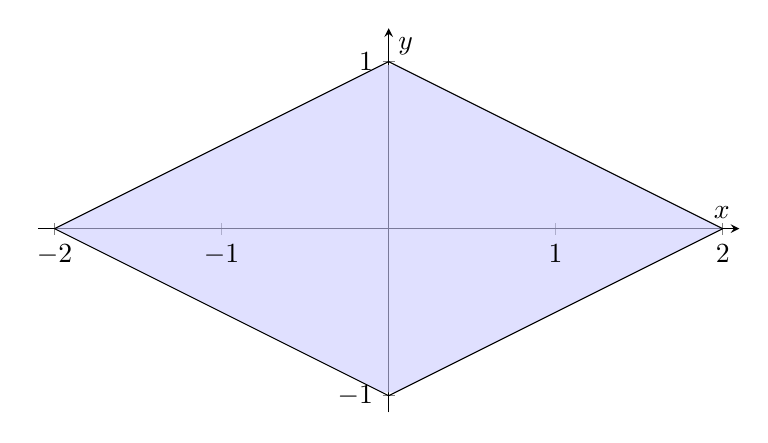
\begin{tikzpicture}
  \begin{axis}[
    axis equal image,
    xlabel=$x$, ylabel=$y$,
    xmin=-2.1, xmax=2.1,
    ymin=-1.1, ymax=1.2,
    xtick={-2,-1,1,2},
    domain=2:2,
    samples=50,
    axis lines=middle,
    clip=true,
    scale=1.3,
    ]
    
    \draw (2,0)--(0,-1); \draw (0,-1)--(-2,0); \draw (-2,0)--(0,1); \draw (0,1)--(2,0);

    \addplot[domain=-2:2,draw=none, name path=A] {1-abs(x/2)};
    \addplot[domain=-2:2,draw=none, name path=B] {abs(x/2)-1};
    \addplot[domain=-2:2, opacity=0.6, blue!20] fill between[of=A and B];

  \end{axis}
\end{tikzpicture}
\end{center}

\newpage

\noindent $\mathrm{F}_1$ and $\mathrm{F}_2$ have continuous partial derivatives. $C$ is a closed curve with positive orientation. We may use the tangential form of Green's Theorem to evaluate the line integral.
\begin{align}\mathrm{I}&=\oint_C\left(x^3\sin\left(\sqrt{x^2+4}\right)-x\mathrm{e}^{x+2y}\right)\,dx + \left(\cos\left(y^3+y\right)-4y\mathrm{e}^{x+2y}\right)\,dy\nonumber\\\nonumber\\&=\iint_R\left(\frac{\partial\mathrm{F}_2}{\partial x}-\frac{\partial\mathrm{F}_1}{\partial y}\right)\,dA=\iint_R\left(-4y\mathrm{e}^{x+2y}\cdot1-\left(-x\mathrm{e}^{x+2y}\cdot2\right)\right)\,dA\nonumber\\\nonumber\\&=\iint_R(2x-4y)\cdot\mathrm{e}^{x+2y}\,dA\end{align}

\noindent From the edges of the parallelogram, we have $\displaystyle x=2y+2,\:x=2-2y,\:x=-2-2y,\:x=2y-2$. Now, use the method of change of variables. Let $\displaystyle u=x-2y,\:v=x+2y$. Then $\displaystyle x=\frac{u+v}2,\quad y=\frac{v-u}{4}$.

\[x=2y+2\implies \frac{u+v}2=2\left(\frac{v-u}4\right)+2\implies u=2\]
\[x=2-2y\implies \frac{u+v}2=2-2\left(\frac{v-u}4\right)\implies v=2\]
\[x=-2-2y\implies \frac{u+v}2=-2-2\left(\frac{v-u}4\right)\implies v=-2\]
\[x=2y-2\implies \frac{u+v}2=2\left(\frac{v-u}4\right)-2\implies u=-2\]

\hfill

\noindent The region in $uv$-coordinates becomes as follows. Calculate the Jacobian determinant and rewrite the integral in $(1)$.

\begin{center}
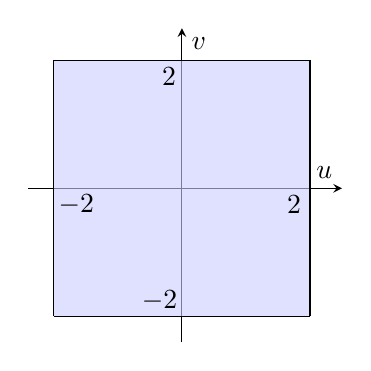
\begin{tikzpicture}
  \begin{axis}[
    axis equal image,
    xlabel=$u$, ylabel=$v$,
    xmin=-2.4, xmax=2.5,
    ymin=-2.4, ymax=2.5,
    xtick=\empty, ytick=\empty,
    domain=2:2,
    samples=50,
    axis lines=middle,
    clip=true,
    scale=0.7,
    ]
    
    \draw (-2,-2)--(-2,2); \draw (-2,2)--(2,2); \draw (2,2)--(2,-2); \draw (2,-2)--(-2,-2);

    \addplot[domain=-2:2,draw=none, name path=A] {2};
    \addplot[domain=-2:2,draw=none, name path=B] {-2};
    \addplot[domain=-2:2, opacity=0.6, blue!20] fill between[of=A and B];

    \node at (-1.65,-0.25) {$-2$};
    \node at (-0.35,-1.75) {$-2$};
    \node at (1.75,-0.25) {$2$};
    \node at (-0.2,1.75) {$2$};

  \end{axis}
\end{tikzpicture}
\end{center}
\[
\frac{\partial(x,y)}{\partial(u,v)}=\left|\begin{array}{cc}
\displaystyle\frac{\partial x}{\partial u}&\displaystyle\frac{\partial x}{\partial v}\\[1em]
\displaystyle\frac{\partial y}{\partial u}&\displaystyle\frac{\partial y}{\partial v}
\end{array}\right|=
\left|\begin{array}{cc}
\displaystyle\frac12&\displaystyle\frac12\\[1em]
\displaystyle\frac{-1}4&\displaystyle\frac14
\end{array}\right|=\frac12\cdot\frac14-\frac12\cdot\frac14=\frac14
\]

\hfill

\begin{align*}\mathrm{I}&=\iint_R(2x-4y)\cdot\mathrm{e}^{x+2y}\,dA=\int_{-2}^2\int_{-2}^22u\mathrm{e}^{v}\cdot\left|\frac{\partial(x,y)}{\partial(u,v)}\right|\,du\,dv=\int_{-2}^2\int_{-2}^22u\mathrm{e}^{v}\cdot\left|\frac14\right|\,du\,dv\\\\&=\int_{-2}^2\mathrm{e}^v\left[\frac{u^2}4\right]_{u=-2}^{u=2}\,dv=\int_{-2}^2\mathrm{e}^v\cdot0\,dv=\boxed0\end{align*}

\end{document}